\documentclass[9pt,twocolumn,twoside]{styles/osajnl}
\usepackage{fancyvrb}
\journal{i524} 

\title{Nagios - Example Paper for I524}

\author[1]{Tony Liu}
\author[1]{Vibhatha Abeykoon}
\author[1]{Gregor von Laszewski}

\affil[1]{School of Informatics and Computing, Bloomington, IN 47408, U.S.A.}


\dates{paper-1, \today}

\ociscodes{Cloud, I524}

% replace this with your url in github/gitlab
\doi{\url{https://github.com/vibhatha/sp17-i524/blob/master/paper1/S17-TS-0003/report.pdf}}


\begin{abstract}
This paper is an example research article for I524, written under the example template. 
We selected Techlist 363, Nagios, as the topic to demonstrate how to properly compose a research
article.
Nagios is a platform/tool, which provides a set of software for system and network infrastructure monitoring. Within this article, we explored what problem it tried to solve, how it solved the problem, and why it's important to have Nagios. We also discussed the advantages and disadvantages it possessed. 
\end{abstract}

\setboolean{displaycopyright}{true}

\begin{document}

\maketitle

\section{Introduction}

According to ~\cite{nagios-book}, even through the machines have become more and 
more critical to us human being, yet they are untrustworthy. We couldn't agree more with the author on this. The newest example on this is the GitLab.com incident happened on Jan 31st 2017. A tired system administrator, working late at night in the Netherlands, had accidentally deleted a directory on the wrong server during a frustrating database replication process: he wiped a folder containing 300GB of live production data that was due to be replicated~\cite{gitlabmeltdown}. Mistakes could be corrected easily since Gitlab have deployed several methods to backup and replicate the production data and all they just need to do is to recover and restore from the backup. However, after several attempts, they found that out of 5 backup/replication techniques deployed none were working reliably or set up in the first place. People haven't emphasize enough about how crucial it is to backup the important data. However, none of this matters if the backup mechanism no long works. That's why we will explore Nagios in this paper.


\section{What is Nagios}

Nagios is a system and network monitoring tool under open source license that provides instant awareness of mission-critical IT infrastructure. Nagios allows to monitor the infrastructure, alert the system admin, provide visualized reports, schedule downtime for maintenance, and plan upgrade in advance with trends and capacity diagrams. Its design emphasizes highly on flexibility and scalability. To provide such flexibility, Nagios is composed of different modules. The reason behind this modular design is that Nagios fully considers the variety of systems and networks it will monitor on. Different customers require a large amount of customization before they themselves know they do.



\section{Why is Nagios Important}

This section discusses why is Nagios important and why we need it.
Elaborate Nagios' features with Gitlab example in the introduction.
Modular. Scalable. Adaptable.

\label{sec:examples}

The sections below show examples of different article components.

\section{Advantages and Disadvantages}

We will dig more on Nagios by take a look at its architecture.

\subsection{Sample Figure}

Figure \ref{fig:nagios-architecture} shows an example figure.

\begin{figure}[htbp]
\centering
\fbox{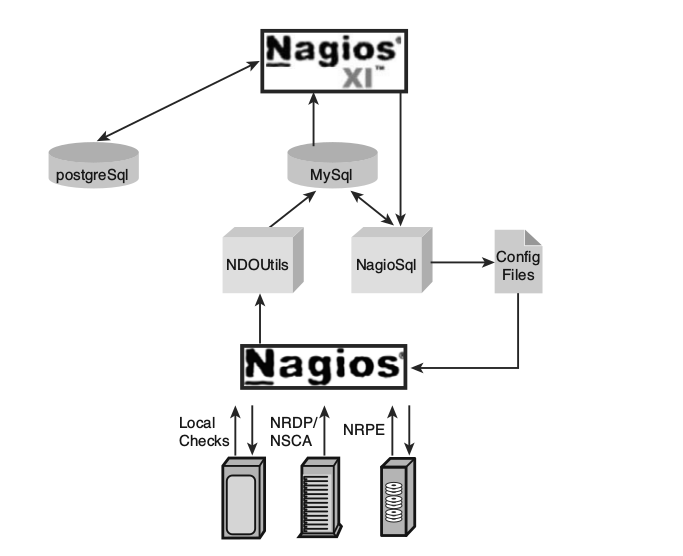
\includegraphics[width=\linewidth]{images/nagios-architecture}}
\caption{Nagios Architecture}
\label{fig:nagios-architecture}
\end{figure}



\section{Conclusion}
Put in some conclusion based on what you have researched.  Use cases,
educational materials can be added to this.  In addition to that ways
Nagios can be improved to get better performance can be included in
your conclusion. With the Gitlab incidence, we can see how
untrustworthy the machines can be. This is also why we need Nagios.



% Bibliography

\bibliography{references}
 
%\newpage

\appendix


\end{document}
